% VDTN, predictivo, replicación, peoabbilista
\subsubsection{MaxProp}
MaxProp\cite{mprop} es un protocolo orientado a redes vehiculares, que considera una restricción en el tiempo y ancho de banda de los contactos. 
Su estrategia se basa en estimar los enlaces con los vecinos asignando pesos, generando un grafo que va aumentando sus pesos según el número de contactos, con lo que se puede estimar el costo de cada camino, como se ve en la Figura \ref{fig:pathcost}. Este cálculo es bastante rápido en la práctica al tener los pesos un aumento monótono.

\begin{figure}[h]
\centering
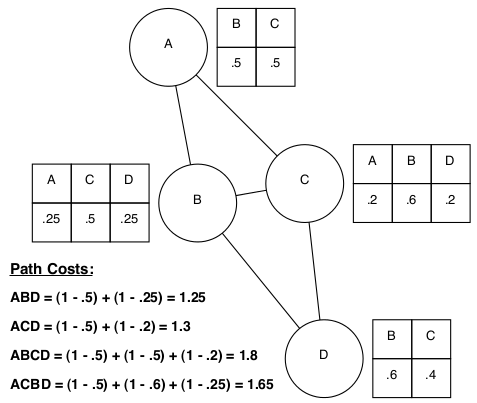
\includegraphics[width=250px]{pathcost.png}
\caption{Cálculo de costos de caminos en MaxProp \cite{mprop}}
\label{fig:pathcost}
\end{figure}

Además, los paquetes a enviar son ordenados según el número de saltos que han realizado, y una vez pasado un cierto umbral, ordenados por la probabilidad de entrega, calculada a partir del grafo. Así, los mensajes se van descartando cuando ya llevan muchos saltos, o cuando su probabilidad de entrega es muy baja, mientras se prioriza el esparcir mensajes nuevos al comienzo, independiente de su probabilidad de entrega.

Al encontrarse dos nodos, intercambian sus cálculos de pesos y los paquetes de mayor prioridad, aumentando el número de saltos de éstos. Los nodos guardan una cantidad considerabled de información de los paquetes que han pasado por él, y cada paquete a su vez guarda información de los nodos por los que ha pasado por lo que se requiere una capacidad de almacenamiento alta, lo que no resulta problemático en redes vehiculares pero potencialmente sí en otros contextos.

MaxProp logra buenos resultados en pruebas usando trazas reales de buses, concluyendo que funciona mejor que el protocolo donde se conocen los encuentros y por tanto el grafo óptimo. En \cite{mprop2} se comparó este algoritmo con Spray and Wait y PRoPHET, usando un movimiento \emph{Shortest
Path Map Based Movement}, donde MaxProp no destacó en rendimiento, y se observó que tiene un gran overhead en sus transmisiones. 